\section{Digitalisierung}

Zu Beginn steht die Herausforderung, ein physisch vorliegendes Puzzle zu digitalisieren.
Eine digitale Version des Puzzles ist einerseits für die Lösungsalgorithmik notwendig, andererseits aber auch zur Visualisierung
der Lösung durch einen simulierten Roboter. Diese Aufgabe wurde vom Team Digitalisierung gelöst.

\subsection[Anfertigung der Rohaufnahmen]{Anfertigung der Rohaufnahmen \myAuthor{Cedric Holzer}}

Vorliegend war ein physisches Puzzle mit 49 Puzzleteilen, von welchem ein möglichst detailgetreues,
digitales Abbild erstellt werden sollte. Dieses soll das physische Original
hinsichtlich Formen und Farben möglichst fehlerfrei abbilden, d.h. ohne
Artefakte wie Schlagschatten an den Kanten, ohne Verzeichnungen und
Verzerrungen und mit möglichst hoher Maßstabstreue.

\paragraph{Fotografie}

Die Puzzleteile wurden einzeln mit einer Digitalkamera vor einem vorbereiteten Hintergrund
möglichst gerade von oben fotografiert. Dabei wurde ein Stativ verwendet, um
die Kameraposition relativ zum Hintergrund konstant zu halten. Soweit möglich
wurden alle Einstellungen der Kamera manuell auf feste Werte gesetzt, um
keine künstlichen Abweichungen zwischen den
Einzelbildern zu erzeugen. Dazu zählen Weißabgleich, ISO-Wert,
Blendenzahl und Belichtungsdauer, aber auch Funktionen wie die
automatische Belichtungsoptimierung, die deaktiviert werden müssen.
Verwendet wurde eine Canon EOS RP Kamera mit einem Canon RF 35mm F1.8
Macro IS STM Objektiv.

\begin{figure}
\centering
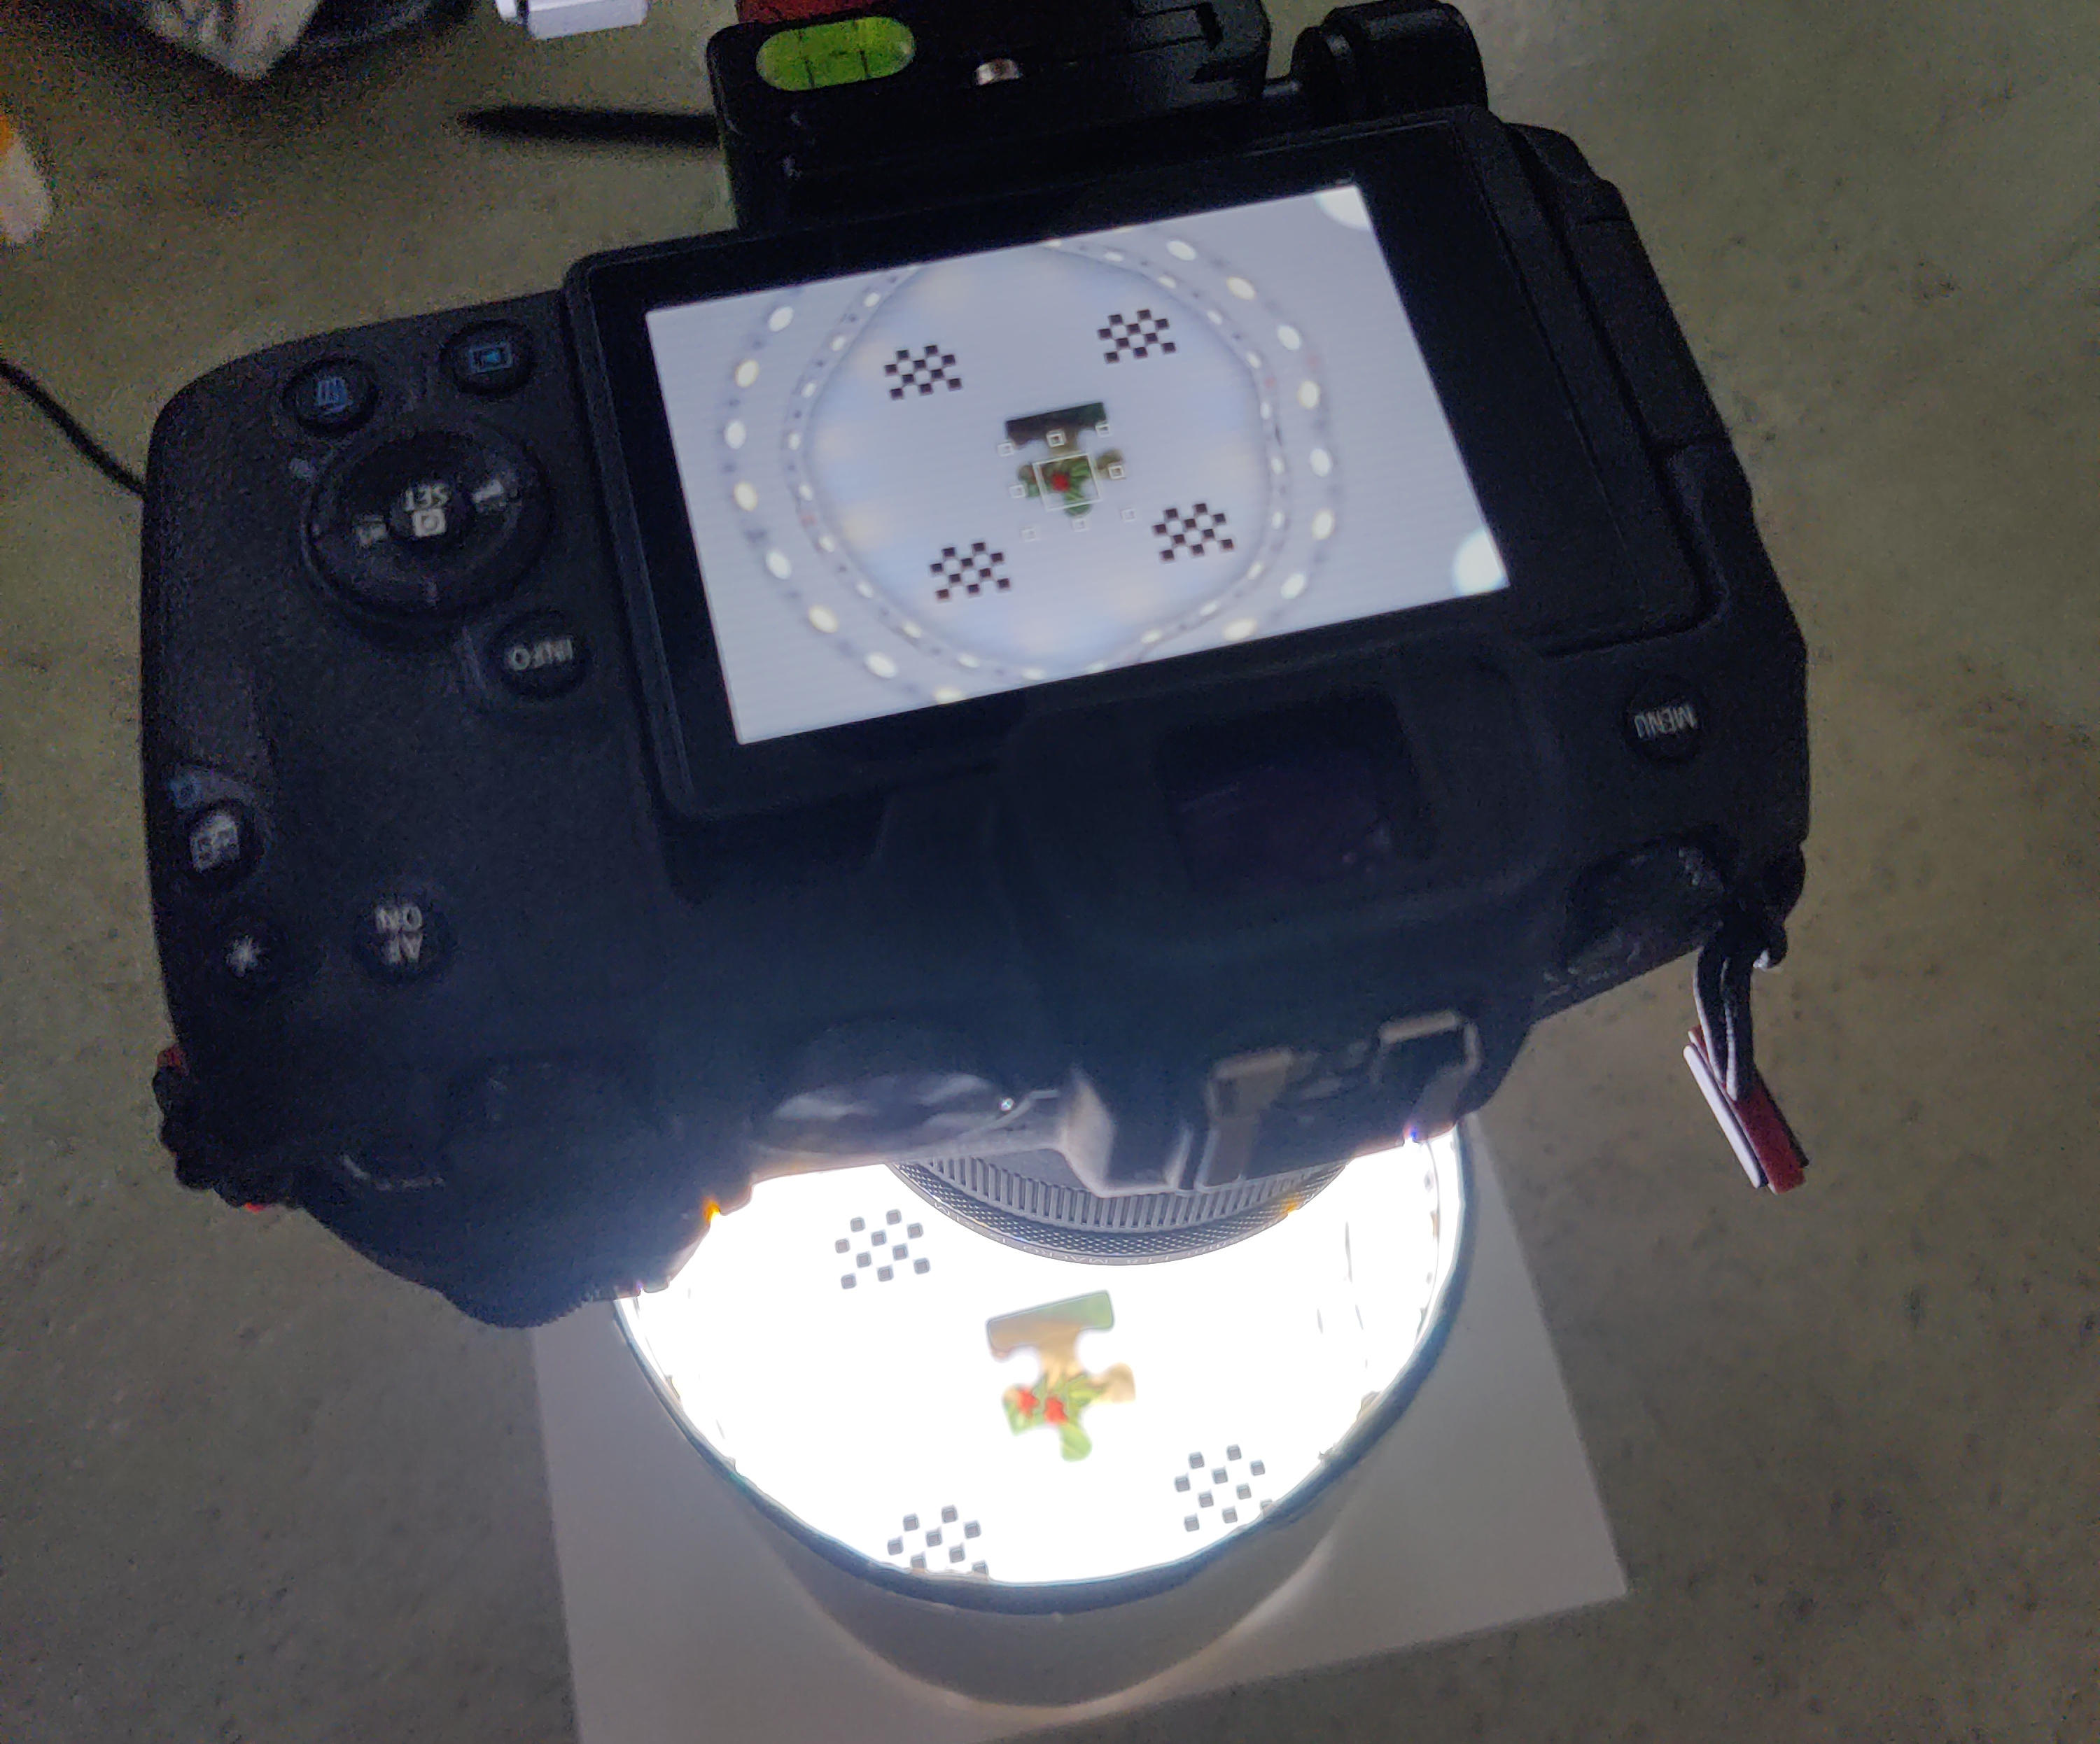
\includegraphics[width=0.6\textwidth]{sections/digitalize/images/foto_setup.jpg}
\caption{Setup zur Fotografie der Puzzleteile mit Stativ, Ringleuchte und Hintergrundgrafik}
\label{fig:foto_setup}
\end{figure}

Um Schlagschatten an den Rändern der Puzzleteile zu vermeiden, ist eine
gleichmäßige Ausleuchtung elementar. Dazu wurde eine provisorische
Ringleuchte verwendet, die aus einem Papierzylinder mit innen
aufgeklebten LED-Streifen besteht. Dieser Papierzylinder wurde so
aufgestellt, dass Puzzleteil und Objektiv sich im Inneren befinden und
so von allen Seiten beleuchtet werden. Der gesamte Aufbau zur Anfertigung der Rohbilder ist
in \autoref{fig:foto_setup} zu sehen. Gut zu erkennen sind die LED-Streifen der Ringleuchte
und die Schachbretter der Hintergrundgrafik. Am oberen Ende ist die Stativhalterung der Kamera zu sehen.

\paragraph{Hintergrund}

\begin{figure}
\centering
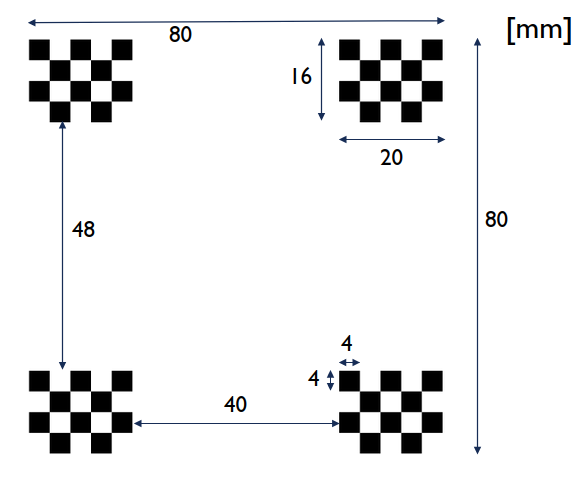
\includegraphics[width=0.6\textwidth]{sections/digitalize/images/background.png}
\caption{Hintergrundgrafik für Aufnahme der Puzzleteile}
\label{fig:background}
\end{figure}

Die in \autoref{fig:background} zu sehende Hintergrundgrafik, vor der alle Puzzleteile
fotografiert wurden, wurde mittels Inkscape erstellt, einer freien Software zur Erstellung
und Bearbeitung von Vektorgrafiken. Die Hintergrundgrafik ist notwendig,
um zusätzliche Informationen über die Aufnahmeperspektive
maschinenlesbar in den Bildern zu kodieren und damit später die
Perspektive korrigieren zu können. Der Hintergrund besteht aus einem
weißen Blatt Papier mit vier schwarz-weißen Schachbrettmustern, deren
äußere Ecken ein Quadrat von 80 mm Seitenlänge aufspannen. Die
Schachbretter bestehen aus 4 Reihen mit je 5 quadratischen Feldern von
4 mm Kantenlänge. Die asymmetrische Form erlaubt die Definition einer
eindeutigen Symmetrieachse. Die Fläche, die von den vier Mittelpunkten
der Schachbretter aufgespannt wird, ist damit ein 60 mm breites und 64 mm
hohes Rechteck mit einem Seitenverhältnis von 15:16.

\paragraph{Entwicklung}

Die Bilder wurden im Format CR3 aufgenommen, einem RAW-Format. Sie
wurden zunächst in ein für die weitere Verarbeitung brauchbareres
Format, nämlich JPG, konvertiert. Dafür wurde die Open-Source-Software
Darktable eingesetzt. In diesem Schritt wurden die Bilder zugeschnitten,
um die sichtbaren Bereiche der Ringleuchte zu entfernen, die nicht von
Interesse sind. Zudem wurde die Verzeichnung der Bilder anhand der vom
Hersteller bereitgestellten und in Darktable enthaltenen Profile für
diese Kamera-Objektiv-Kombination korrigiert. Der Darktable-Stil, eine Art Protokoll
der vorgenommenen Schritte, ist zur Reproduzierbarkeit dieses manuellen Vorgehens
im digitalizer-Repository zu finden.

\begin{figure}
\centering
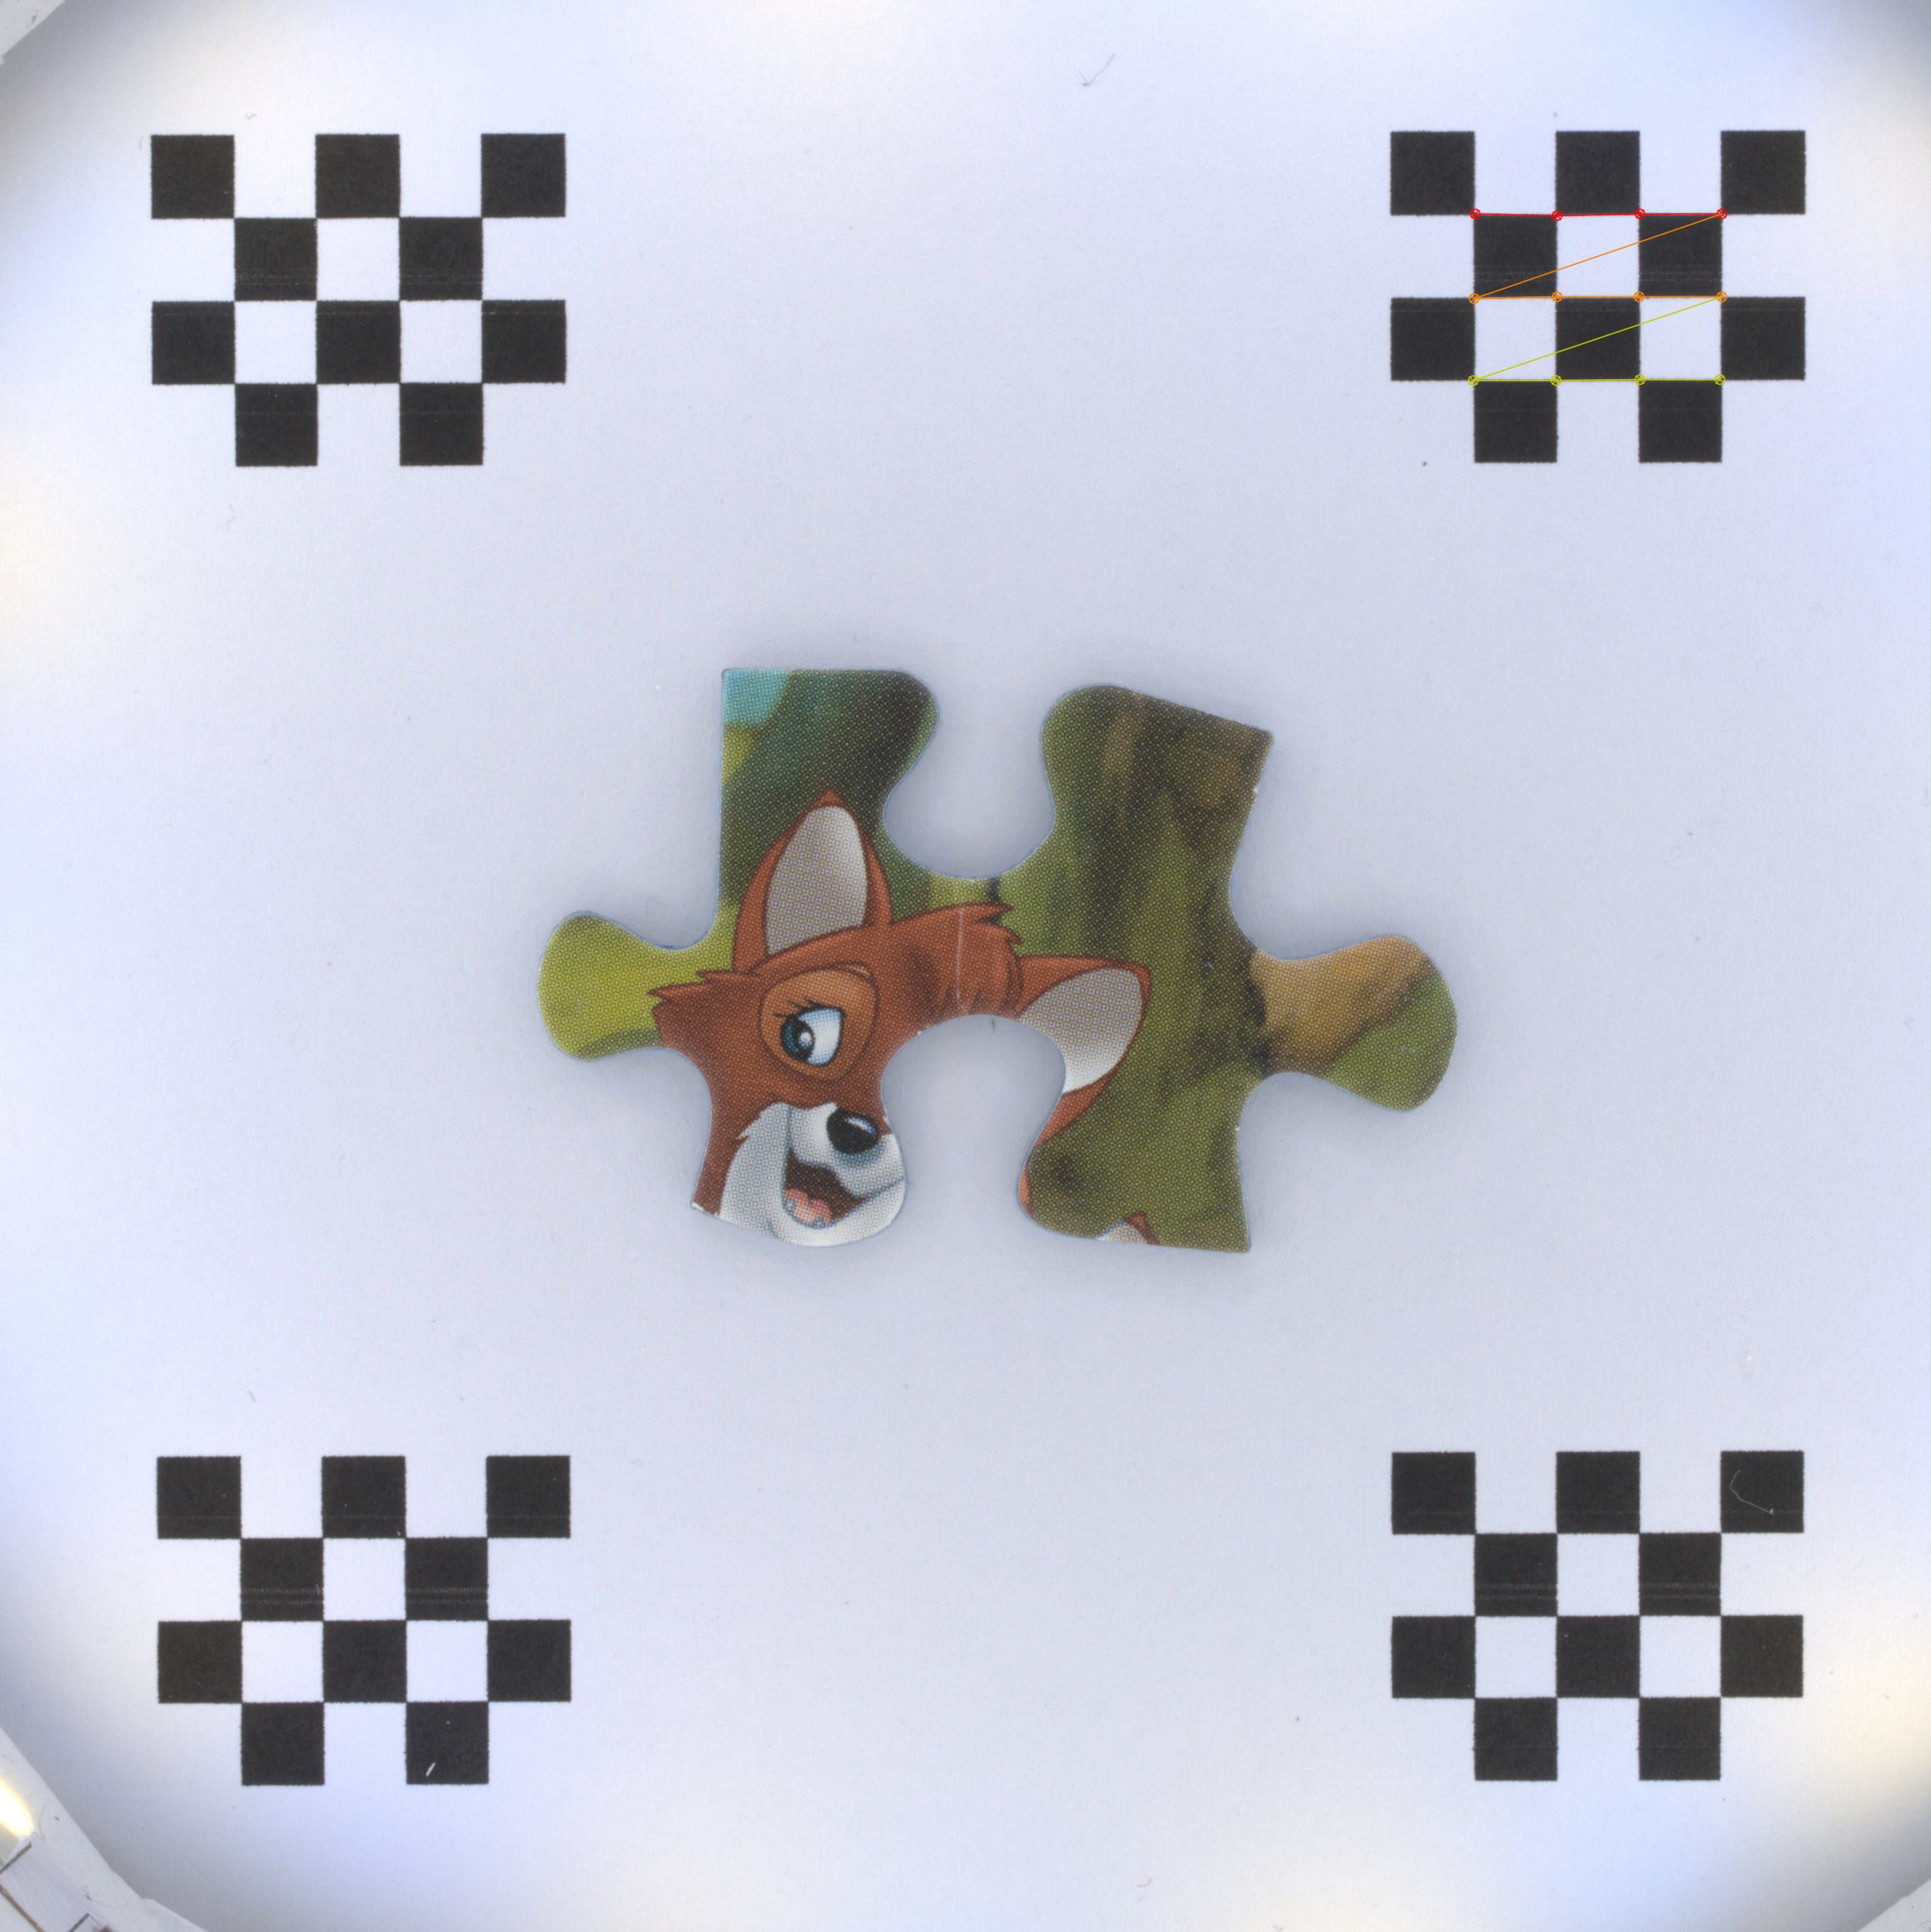
\includegraphics[width=0.6\textwidth]{sections/digitalize/images/example_image_raw.jpg}
\caption{Beispiel eines Bilder nach dem Entwicklungsschritt}
\label{fig:raw_image}
\end{figure}

\autoref{fig:raw_image} zeigt ein exemplarisches Foto eines Puzzleteils nach dem Entwicklungsschritt.
Das Bild ist so zugeschnitten, dass Teile der Ringleuchte großteils entfernt wurden, die Schachbretter
aber noch vollständig und mit etwas Rand sichtbar sind.

\subsection[Perspektivische Korrektur]{Perspektivische Korrektur \myAuthor{Cedric Holzer}}

Im nächsten Schritt wird die Perspektive der Bilder korrigiert. Dadurch
werden einerseits alle Bilder auf einen exakt identischen Maßstab
skaliert und andererseits werden Verzerrungen beseitigt, die durch eine
nicht parallele Ausrichtung von Sensor- und Motivebene entstehen können.

Für die Perspektivkorrektur ist es notwendig, vier Punkte in einem Bild
zu erkennen, deren Lage im abgebildeten Raum bekannt ist. Für diesen
Zweck bestehen die Schachbrettmuster im Hintergrundbild. Deren innere
Kreuzungspunkte, d.h. Punkte, an denen sich vier benachbarte Felder des
Schachbretts treffen, können mittels der Funktion
\texttt{cv2.findChessboardCorners} erkannt werden, die in der
Bildverarbeitungsbibliothek OpenCV enthalten ist. Sie findet ein
Schachbrett definierter Größe in einem Bild. Damit dieser Schritt
korrekt funktioniert, werden die Bilder zunächst in einem
Vorbereitungsschritt leicht aufgehellt und stark kontrastverstärkt,
sodass die Schachbretter fast nur aus reinen Schwarz/Weiß Pixeln
bestehen.

Da ein Bild vier Schachbretter beinhaltet, OpenCV aber nur eines pro
Bild detektiert, wird das Bild zunächst in vier Viertel geteilt, in
welchen separat nach dem jeweils enthaltenen Schachbrett gesucht wird.
Die gefundenen Koordinaten der Schachbretter müssen anschließend wieder
in das Koordinatensystem des Ursprungsbildes zurückgerechnet werden.

Die Koordinaten der Kreuzungen jedes Schachbrettes werden gemittelt,
sodass sich vier Mittelpunkte pro Bild ergeben. Da auf den
perspektivisch noch nicht korrigierten Bildern gemittelt wird, verzerrt
dieser Schritt die vier Mittelpunkte unterschiedlich. Sollte sich die
Perspektive der Bilder stark unterscheiden, dürfte es vorzuziehen sein,
nur den äußersten Punkt jedes Schachbretts zu verwenden ohne zu mitteln.
Dieses Vorgehen wäre verzerrungsfrei, dafür aber anfälliger für ungenau erkannte
Kreuzungskoordinaten. Durch die Verwendung eines Stativs ist die
Perspektive in unserem Fall fast konstant und die Sensorebene annähernd
parallel zur Motivebene. Damit ist nur eine leichte Verzerrung zu
erwarten, die für alle Bilder annähernd identisch ist.

\begin{figure}[h!]
    \centering
    \begin{minipage}[b]{0.5\textwidth}
        \centering
        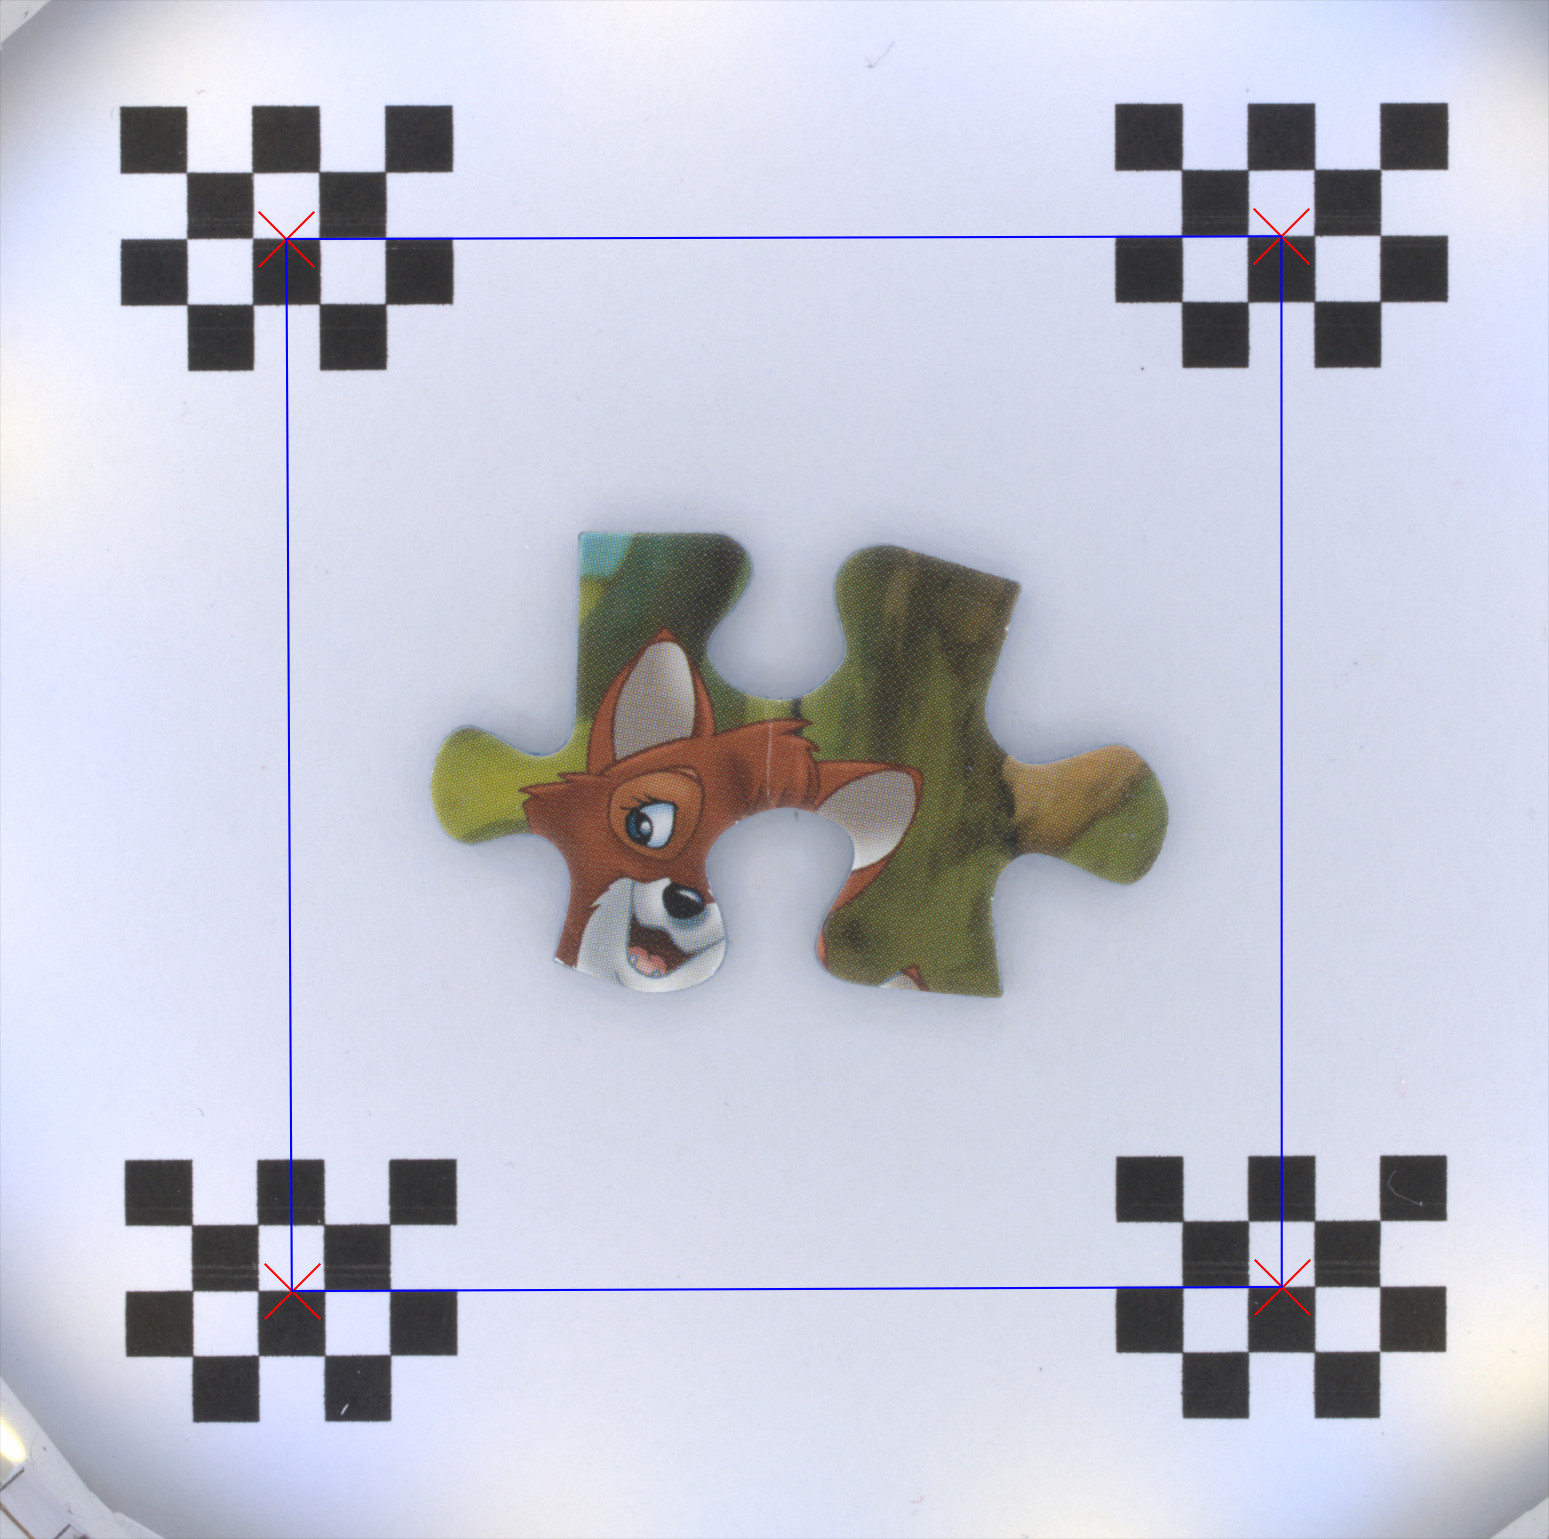
\includegraphics[width=\textwidth]{sections/digitalize/images/rectification_recognized.jpg}
    \end{minipage}
    \hfill
    \begin{minipage}[b]{0.4\textwidth}
        \centering
        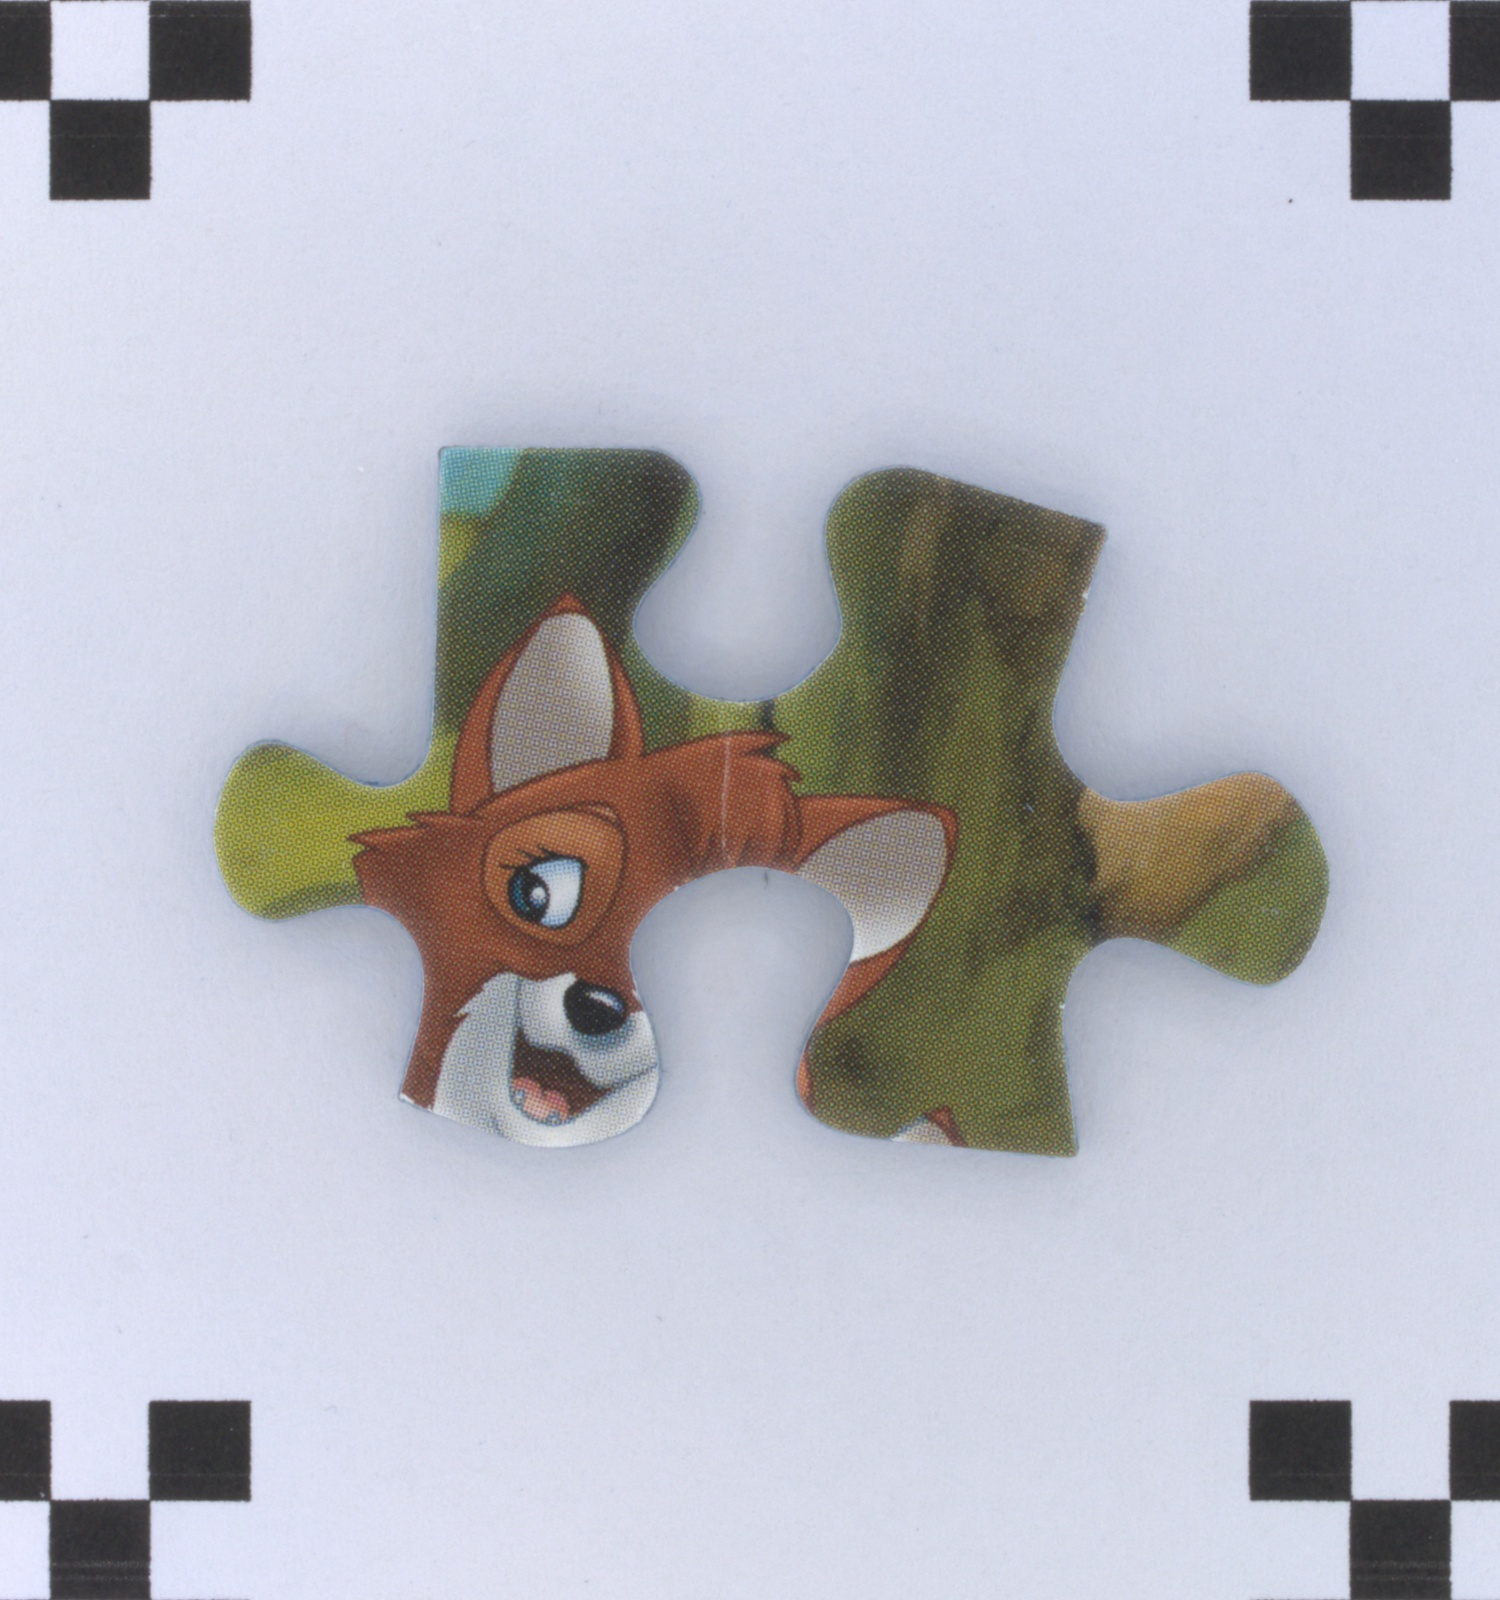
\includegraphics[width=\textwidth]{sections/digitalize/images/rectification_done.jpg}
    \end{minipage}
    \caption{Erkannte Abbildungsfläche im unkorrigierten Bild (links) und Resultat der Perspektivkorrektur (rechts)}
    \label{fig:rectification_result}
\end{figure}

Die realen Abstände der ermittelten vier Mittelpunkte sind bekannt. Ein Beispiel für diesen Schritt ist in
\autoref{fig:rectification_result} zu sehen. Die vier Mittelpunkte der Schachbretter
spannen im unkorrigierten Bild ein Parallelogramm auf, das nun in ein
1500px x 1600px Rechteck transformiert wird. Dabei werden die ermittelten Mittelpunkte in
die Ecken des Bildes verschoben. Das abgebildete Rechteck entspricht einer realen Fläche von
60mm x 64mm, was einen Maßstab von $1mm=25px$ beziehungsweise $1px=40\mu{}m$ ergibt.

\paragraph{Implementierung}

Der Darktable-Stil zur Entwicklung der Rohbilder sowie die SVG-Datei des
Hintergrunds liegen im digitalizer-Repository im \texttt{/resources}
Ordner. Zur perspektivischen Korrektur aller Bilder in einem Ordner kann im selben Repository das
Python-Skript \texttt{src/rectification/rectification.py} verwendet
werden.

\subsection{Segmentierung}

% Einleitung Segmentierung
Durch das Pre-Processing werden also aus den fotografierten Puzzleteilen, linear entzerrte und einheitlich zugeschnittene JPG Bilder generiert, wie in Abbildung \ref{fig:lrcpt} dargestellt.
Diese dienen als Eingabe für den nächsten Schritt, die \textit{Segmentierung}.

% Was ist Segmentierung und wieso
Bei der Segmentierung werden zusammenhängende Strukturen in einem Bild erkannt und die entsprechenden Pixel dem Vordergrund bzw. dem Hintergrund zugeordnet.
Dabei entsteht verbunden binäre Bildregionen, welchen im Weiteren die Form eines Objektes bzw. in diesem Fall des Puzzleteils beschreiben \cite{burger2009digitale}.
Anhand der Form kann der Solver später zum Beispiel Kanten- und Color Matching vornehmen.

% Aufgabe
Aufgaben ist nun, diese Puzzleteile zu erkennen und an den Kanten auszuschneiden bzw. den Hintergrund zu entfernen.
Dafür wurden zwei verschiedene Ansätze exploriert, wobei einer ausschließlich auf digitale Bildverarbeitungsmethoden zurückgreift, während die andere eine Künstliche-Intelligenz (KI) beinhaltet.
Beide Ansätze benutzen dabei die gleichen Bilder als Basis.
Diese werden im Folgenden beschrieben.

\begin{figure}[h]
    \centering
    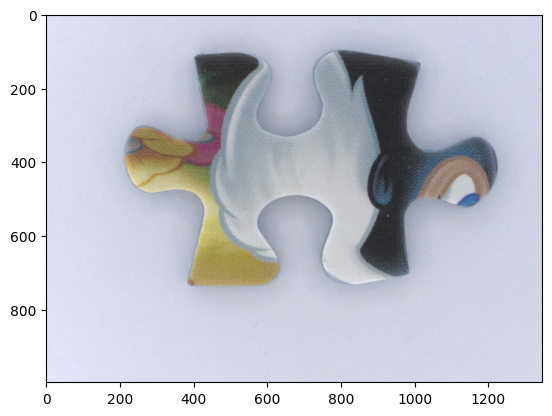
\includegraphics[width=0.4\textwidth]{sections/digitalize/images/org_8647.png}
    \caption{Linear entzerrtes und zugeschnittenes Puzzleteil}
    \label{fig:lrcpt}
\end{figure}

\subsubsection[Segmentierung mit digitaler Bildverarbeitung]{Segmentierung mit digitaler Bildverarbeitung \myAuthor{Kipp}}
% Einleitung IP
Die digitale Bildverarbeitung bietet einen großen Werkzeugkasten an bekannten und bewährten Algorithmen für Bildmanipulation und Transformation.
Die nachfolgend dargestellte Segmentierungsmethode stützt sich ausschließlich auf diese Werkzeuge und kommt dabei ganz ohne künstliche Intelligenz aus.
% Vorteile von IP
Das hat den Vorteil, dass diese selbst auf schwacher Hardware zielführend genutzt werden kann.
Die genutzten Algorithmen etwa zur Konvertierung der Farbräume, der Faltung von Bildern mit einem Kernel oder das Finden von Kanten sind schon lang bekannte und daher gut optimiert, dokumentierte und in diversen Quellen hinreichend nachvollziehbar erklärt.
Da es sich um konkrete Anleitungen handeln, wie die Pixel in einem Bild verarbeitet werden müssen, ist kein vorheriges Trainieren bzw. Lernen eines Models notwendig, die Abarbeitung der statischen Instruktionen ist ausreichend.
Daher ist der Output deterministisch, da stets bei gleicher Eingabe, die gleiche Ausgabe zu erwarten ist.

\paragraph{Segmentierungsansätze}
% Mögliche Alternative Ansätze, Watershed und & Threshold
In der Bildverarbeitung gibt es nicht die \textit{einen} Methode, um Objekte von einem Hintergrund zu segmentieren.
Die Wahl des Vorgehens hängt von der Aufgabe ab und wie gut eine Methode auf dem gegebenen Problem performt.
Grob lassen sich Segmentierungsansätze in zwei Kategorien unterteilen.
Diese lassen sich selbst wiederum unterteilen \cite{kaur2014various}.

Diese Klasse an \textit{Similarity-Based} Verfahren segmentiert Regionen basierend auf der Ähnlichkeit seiner Pixel.
Darunter fallen alle \textit{Thresholding} und \textit{Region Growing Techniques} wie der \textit{Watershed} Algorithmus.

Thresholding Methoden teilen die Pixel in einem Bild nach ihrem Helligkeitswert anhand eines Schwellwertes in Vorder- und Hintergrund ein.
Sie funktionieren gut, wenn das Objekt heller ist als der Hintergrund.

% wie lief es im projekt
Für das Puzzleprojekt wurde in einer frühen Phase ein adaptiver Threshold für die Segmentierung verwendet.
Bei dem adaptiven Threshold wird kein globaler Schwellwert, welcher sehr anfällig für Schatten ist, sondern mehrere regionale Schwellwerte verwendet, welche robuster gegen Lichteinfluss sind.
Die Eingabe Bilder sind gut, aber nicht perfekt ausgeleuchtet, so zeigt das Ergebnis ein grundsätzlich richtig segmentiertes Puzzleteil, jedoch mit noch zu vielen Schatten an den Rändern wie in Abbildung \ref{fig:segment_ergebnis}.

Das Watersehd Verfahren interpretiert die Pixel und ihren Gradienten der Helligkeit in einem monochromen Bild als Höhenkarte.
Dabei stellen lokale Minima Täler dar, welche mit Wasser geflutet werden.
Der Wasserspiegel steigt und trifft auf andere Täler bzw. Wasseransammlungen, welche dann vereint werden.
Um Regionen separat voneinander zu halten, werden Dämme als Grenzen eingesetzt.
Diese Dämme werden mittels Dilatation ermittelt.
Je höher der Gradient eines Pixels, desto eher handelt es sich um einen Damm.

% wie lief es im projekt
Auch diese Methode wurde für das Puzzleprojekt evaluiert und hat aber mit den gewählten Parametern und der gewählten Umsetzung keine Puzzleteile segmentiert, sondern die Objekte auf den Puzzleteilen unterteilt, wie in Abbildung \ref{fig:segment_ergebnis} zu sehen.
Die Unterteilung war also zu fein und hätte gröber sein müssen.
Es ist anzumerken, dass das keine allgemein gültige Aussauge ist und das Problem hätte mit mehr Recherche und anderen Parametern mit Sicherheit behoben werden können, was eine bessere Segmentierung erlaubt hätte.
In Anbetracht der kurzen Projektdauer und der Tatsache, dass andere Projektkomponenten auf den segmentierten Bildern aufbauen, ist ein anderes, einfacheres, Segmentierungsverfahren gewählt worden.

Diese Klasse an \textit{Discontinuity-Based} Verfahren basiert auf der Annahme, dass Regionen und Segmente in einem Bild durch abrupte Änderungen der Helligkeitswerte bestimmt werden können.
Diese werden meist auf \textit{monochromen}, also einfarbigen Bildern, angewendet.
Die Kantenerkennung spielt dabei eine entscheidende Rolle, da Kanten als signifikante Übergänge in der Helligkeit definiert werden können.
Methoden zur Kantenerkennung betrachten den Gradienten, also die Ableitung der Helligkeitsänderung in x und y Richtung.
Die dadurch gewonnen Stärke und Richtung der Kante hilft bei der Identifizierung von relevanten Kanten und Konturen des Puzzleteils.
Solche Techniken nutzt zum Beispiel der \textbf{Canny Edge Detector}, welcher im weiteren Verlauf beschrieben, angewendet und evaluiert wird.

% Gewählter Ansatz: Canny -> Vorgehen und Umsetzung
\paragraph{Segmentierung mit Canny Edge Detector}
Um schnell Prototypen entwickeln und testen zu können und weil alle vorher genannten Methoden als Bibliotheken verfügbar sind, ist Python als Programmiersprache für die Umsetzung der Puzzleteilsegmentierung gewählt worden.
Für die eigentliche Bildverarbeitung werden die Packages \verb|openCV| \cite{opencv_library} und \verb|Pillow| \cite{clark2015pillow} verwendet.

Da die Image Processing Segmentation Klasse (\verb|ip_segmentation.py|) später neben einer KI Segmentation Klasse (\verb|sam_segmentation.py|) in einen ROS2 \cite{scirobotics.abm6074} Node Eingebungen werden soll, wurde die Segmentierungsfunktion gekapselt und stellt eine einzelne, public Funktion \verb|segment(input_image_path: str) -> (list, list)| bereit, welche nur den Pfad zu den Eingabebildern benötigt und nach Abarbeitung eine Liste an segmentierten Bildern und eine Liste an Kanten zurückgibt.
Die \verb|segment(...)| Funktion liest die 49 JPG Bilder ein und wendet die nachfolgend beschriebenen Verarbeitungsschritte zur Ausschneidung des Hintergrunds an.

% 1. Read input image
Zu Beginn wird das Bild als Numpy-Array mithilfe der \verb|Image.open()| Funktion von Pillow als \verb|RGBA| geöffnet.
Der vorher nicht vorhandene vierte Alpha-Kanal wird mit voller Deckkraft hinzugefügt.
Das Numpy Array hat die Shape \verb|(998, 1347, 4)|, das heißt ein Bild wird durch vier Matrizen, drei Farbkanäle und ein Alphakanal, mit den Dimensionen 988 × 1347 dargestellt.

% 2. convert to gray scale
Die auf Kantenerkennung basierende Segmentierung funktioniert am besten auf einfarbigen Bildern.
Für die Farbraumkonvertierung von RGB zu Graustufen, wird die openCV Funktion \verb|cvtColor()| verwendet.
Intern wird dabei für jedes Pixel aus den drei Farbkanälen gewichtet eine Helligkeit ermittelt.
Die Gewichtung der Farben ist orientiert an der Farbwahrnehmung des menschlichen Auges.
Die zurückgegebene Matrix enthält die gleichen Dimensionen aber nur noch einen Kanal, siehe Abbildung \ref{fig:ip_grayscale}.

\begin{figure}[h]
    \centering
    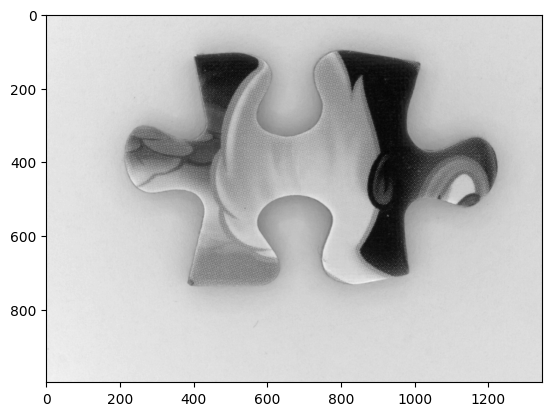
\includegraphics[width=0.4\textwidth]{sections/digitalize/images/gray_8647.png}
    \caption{Graustufen des Puzzelteils}
    \label{fig:ip_grayscale}
\end{figure}

% 3. Canny
Als nächstes wird der Canny Edge Detector auf das Graustufenbild angewendet.
Auch dafür stellt openCV eine Funktion \verb|canny()| bereit.
Der Canny Detector beseht aus mehreren Schritten und hebt Kanten, also abrupte Helligkeitsänderungen hervor.
Zuerst wird mit einem Gausfilter Rauschen auf dem Eingabebild unterdrückt, indem jedes Pixel durch eine Gaußsche Verteilung gewichtet gemittelt wird.
Das reduzierte Rauschens hilt, falsche Kanten zu unterdrücken.
Danach wird ein Sobel Filter horizontal und vertikal über das Bild geschoben um die erste Ableitung zu berechnen.
Die Gradientrichtung und -Stärke können dann aus den Pixeln der Ausgabebildern berechnet werden.
Im dritten Schritt werden nicht-Maximalen Werte unterdrückt.
Hierzu werden entlang der Gradientenrichtung nach lokalen Maxima gesucht, welche behalten werden.
Das führt dazu, dass breite Kanten auf einen Pixel Breite verjüngt werden.
Zum Schluss wird ein Hystersis Thresholding, also ein doppelter Schwellwert, angewendet um schwache Kanten und Rauschen rauszufiltern.
Eine Kante unterhalb des unteren Schwellwerts oder zwischen dem oberen und unteren Schwellwert werden nicht weiter berücksichtigt.
Nur starke Kanten, auch wenn sie nicht durchgehend über dem oberen Schwellwert sind, werden behalten \cite{mordvintsev2014opencv}.
Die min und max Schwellwerte müssen der Canny-Funktion übergeben werden.
Durch experimentelle Annäherung konnten die Werte 20 und 110 ermittelt werden.
Die Ausgabe des Cannys ist also eine Binärbild, wie in Abbildung \ref{fig:canny_canny}, welches ausschließlich starke Kanten beinhaltet.
Zu beachten ist, dass sowohl die Konturen des Puzzleteils als auch jegliche Kanten des Motivs darstellen, enthalten sind.
Die tatsächliche Kantenextraktion des Puzzelteils erfolgt in einem späteren Schritt.

\begin{figure}[h]
    \centering
    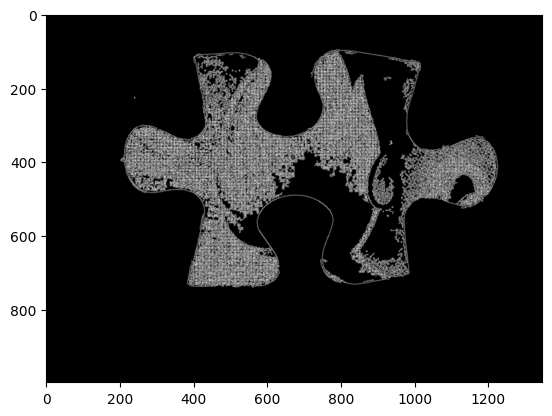
\includegraphics[width=0.4\textwidth]{sections/digitalize/images/canny_canny_8647.png}
    \caption{Verbesserte Kanten mit Canny Edge Detector}
    \label{fig:canny_canny}
\end{figure}

% 4. Blur
Da der Canny Edge Detector nur starke Kanten in Form eines Binärbildes übrig lässt, kann es sein das die Kante, welche die Kontur des Puzzelteils darstellt, um wenige Pixel unterbrochen ist.
Würde jetzt eine Kantenextraktion durchgeführt werden, könnte die gesuchte Kontur nicht gefunden werden.
Aus diesem Grund wird das Binärbild vorher noch Weichgezeichnet.
Bei dem Blur Filter in diesem Fall handelt sich um einen einfachen Durchschnitt, das heißt jeder Pixel nimmt den gemittelt Wert seiner unmittelbaren Umgebung an.
Dadurch wird erreicht, dass im Historgram wieder Graustufen zwischen 0 und 255 zu sehen sind und kleiner Lücken in den Kanten geschlossen werden.

% 5. find contours
Die \verb|findContours()| Funktion findet zusammenhängende Konturen in Bildern.
Konturen können als Grenzen einer Form mit selben Helligkeitswert bezeichnet werden.
Intern wird eine Form des \textit{Border-Follow-Algorithm} verwendet.
Dieser wandelt zuerst das Bild wieder mit einem Threshold wieder in ein Binärbild um, um dannach zeilenweise Pixel für Pixel nach eine vordergrund Pixel zu suchen.
Wenn eins gefunden wurde, wird dieses als Startpunkt markiert und die Nachbarschaft nach ebenfalls vordergrund Pixeln durchsucht.
Dieser Prozess wird solang wiederholt, bis der Startpunkt wieder erreicht ist.
Die Ausgabe ist eine Liste an geschlossenen Kanten.
Die gesuchte Kontur vom Puzzelteil ist die Kontur welche den größten Flächeninhalt einspannt.
Also wird mit einer weiteren OpenCV Funktion \verb|contourArea()| nach der größten Fläche gesucht.
Mit der Gaußschen Trapezformel lässt sich der Flächeninhalt von beliebigen Polygonen bestimmen.
Da nur die eine Kontur für das Projekt relevant ist, werden die anderen gefunden Konturen nicht weiter beachtet.
Die Aufgetragen Kontur auf das Originalbild ist in Abbildung \ref{fig:canny_unsmooth} zu sehen.

\begin{figure}[h]
    \centering
    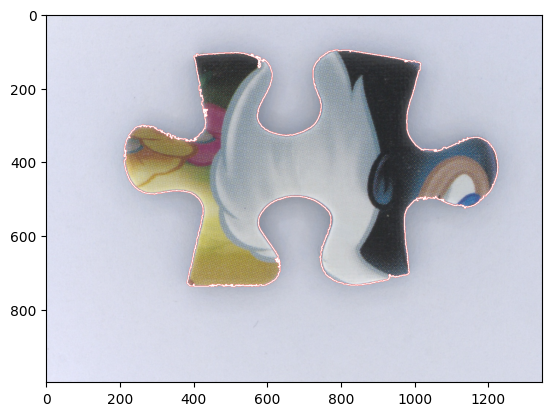
\includegraphics[width=0.4\textwidth]{sections/digitalize/images/canny_unsmoothened_8647.png}
    \caption{Nicht geglätette Kontur}
    \label{fig:canny_unsmooth}
\end{figure}

% 6. blur & "fill" and contours on original
Ein finaler Median-Blur glättet die noch teilweise unsauberen Kanten, wie in Abbildung \ref{fig:segment_ergebnis} zu sehen.

\paragraph{Fazit}
% Ergebnis

\begin{figure}[h]
    \centering
    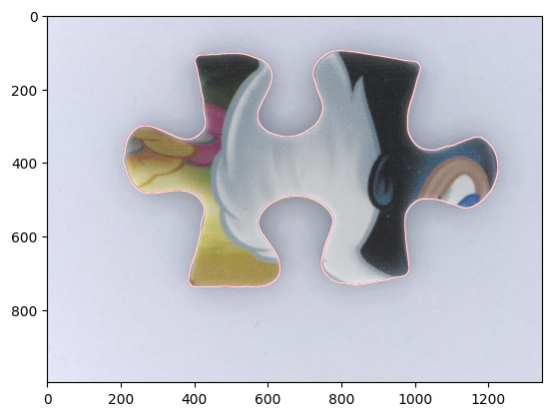
\includegraphics[width=0.4\textwidth]{sections/digitalize/images/canny_final_8647.png}
    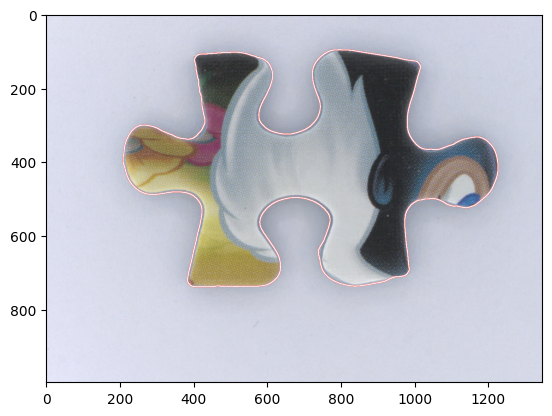
\includegraphics[width=0.4\textwidth]{sections/digitalize/images/thresh_final_8647.png}
    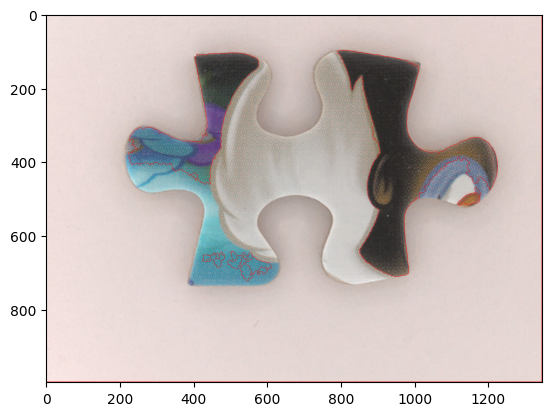
\includegraphics[width=0.4\textwidth]{sections/digitalize/images/water_final_8647.png}
    \caption{Segmentierung - Canny (links), Threshold (rechts), Watershed (unten)}
    \label{fig:segment_ergebnis}
\end{figure}

Zusammenfassend kann festgestellt werden, dass die aufgeführte Segmentierungsmethode basierend auf den Canny Edge Detector für jedes 49 Puzzleteile zuverlässig funktioniert.
Bei genauer Betrachtung fällt allerdings auf, dass immernoch einge Fransen vorhanden sind und Schattige stellen falsch Segmentiert werden.
% !! bild??
Im Vergleich mit der Threshold Methode werden dennoch deutlich mehr Schatten herausgefiltert.
Die Watershed Methode hat durch die falsche Parameterwahl auch schlechter Ergebnisse geliefert.
Für eine bessere Segmentierung sollte das Watershed Verfahren nocheinmal beleuchtet werden.

% Aber, Solver Algorithmus kann das Puzzle auch mit diesen Bildern lösen.
Trotz der Störungen ist es dem Solver aber möglich, das Puzzle mit den ausgabebildern zu lösen.

% Nachteil: hängt AI Methode hinterher
Noch bessere Ergebnisse erziehlt der nachfolgende Segmentierungsansatz mit KI.

\subsubsection[Segment Anything Model (SAM) ]{Segment Anything Model (SAM) \myAuthor{Then}}

% explain SAM being the KI method and a intro to what it is
Segment Anything Model (SAM) ist die KI-Alternative, die zum Segmentieren von Puzzleteilen verwendet wird. SAM ist ein neues KI-Modell von Meta AI, das jedes beliebige Objekt in jedem Bild "ausschneiden" kann, wenn es die gewünschte Eingabe erhält. SAM ist ein Zero-Shot Segmentierungssystem, das sich ohne zusätzliches Training auf unbekannte Objekte und Bilder generalisieren lässt. Mit über 1 Milliarde Masken auf 11 Mio. lizenzierten und die Privatsphäre respektierenden Bildern ist SAM so konzipiert und trainiert, dass es prompt auf neue Bildverteilungen und Aufgaben übertragen werden kann \cite{kirillov2023segment}. Zero-Shot ist ein maschinelles Lernszenario, bei dem ein KI-Modell darauf trainiert wird, Objekte zu erkennen und zu kategorisieren, ohne sie zuvor gesehen zu haben, bzw. ohne dass das Modell zuvor auf die Objekte trainiert wurde \cite{ibm_zero_shot}. SAM wurde als KI-Modell wegen seiner erstaunlichen Zero-Shot-Fähigkeiten ausgewählt, da das Modell auf einem riesigen Datensatz trainiert wurde. Daraus ergibt sich die Frage, ob SAM-Vorhersagen ein akzeptables Segmentierungsergebnis liefern können, ohne dass das Modell für die Segmentierung von Puzzleteilen trainiert werden muss.

% Goal: set up an automated process with SAM to input our rectified puzzle pictures as inputs and output the two different types of expected output as mentioned in the problem section. 
Um die Frage zu beantworten, muss ein angepasster Prozess eingerichtet werden, der den gewünschten Output liefert. Es muss ein Automatisierungsprozess eingerichtet werden. Es gibt zwei Methoden zur Integration von SAM in den Automatisierungsprozess: die lokale Installation der erforderlichen Pakete oder die Durchführung über Cloud-Computing-Dienste wie Google Colab. Für dieses Projekt wurde die letztere Methode gewählt und ein Jupyter-Notebook entwickelt, um SAM in die Lösung zu integrieren. Colab nutzt eine Jupyter-Notebook-Umgebung, die auch \verb|Python| als Kernel verwendet. SAM kann nun heruntergeladen und abgeleitet werden.

%Figure of the bounding region here:
\begin{figure}[h]
    \centering
    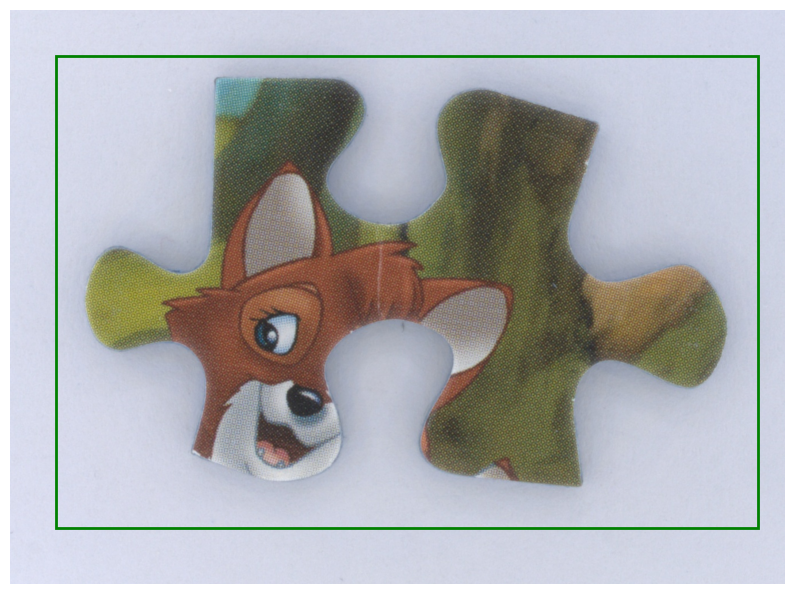
\includegraphics[width=0.4\textwidth]{sections/digitalize/images/SAM_bounding_box_example.png}
    \caption{Bounding Box Region}
    \label{fig:bounding_box_example}
\end{figure}

% SAM methods: SAM requires certain parameters in order to be able to use the model. The important parameters are: Model checkpoints to use, forms of input, and the option to receive a multimask output. 
SAM bietet eine Reihe von Segmentierungsfunktionen, aber die in diesem Projekt verwendete ist der \verb|SamPredictor|. Dies ermöglicht die Verwendung der Funktion \verb|predict|, die vor der Inferenz bestimmte Eingabeparameter erfordert. Zu Beginn muss SAM mit dem trainierten Modell initialisiert werden. Die entscheidenden Parameter sind dann das Eingabeformat zur Aufforderung einer Auswahlregion und die Option einer Multimask-Ausgabe. Im Rahmen der Segmentierung wurde ein Eingabeformat verwendet, das einer Bounding Box folgt, welche einem NumPy-Array entspricht. Dieses Format wurde eingesetzt, um die Region des Bildes zu bestimmen, in der die Segmentierung durchgeführt werden soll. Dadurch wurde das Modell angewiesen, den in diesem Bereich erzielten Ergebnissen mehr Gewicht zu verleihen. Alternativ hätten auch die Pixelpunkte auf dem Bild verwendet werden können, um die gewünschte Segmentierung zu markieren. Diese Vorgehensweise wurde jedoch nicht gewählt, da das Modell dazu tendiert, die feineren Merkmale auf den Puzzleteilen zu segmentieren, wie beispielsweise die auf dem Puzzleteil vorhandenen Bilder.

%Figure of outputs here
\begin{figure}[h]
    \centering
    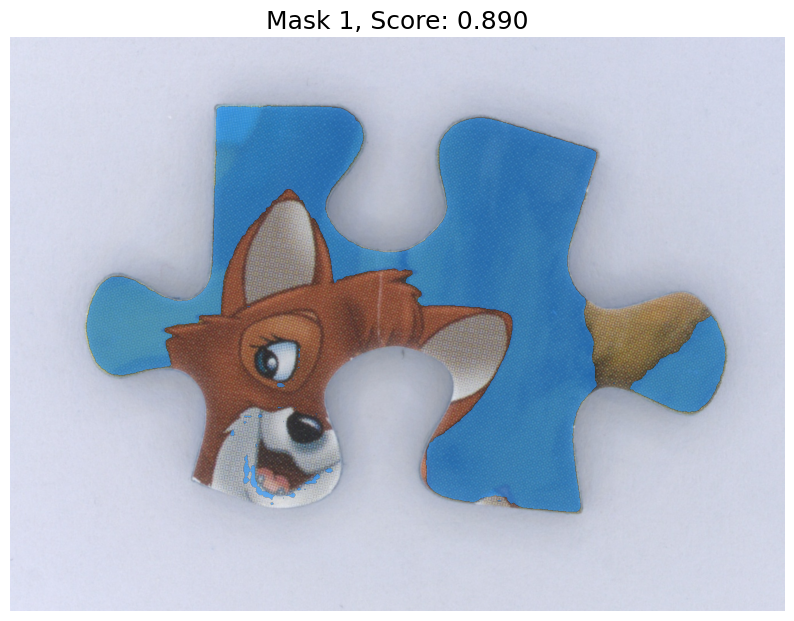
\includegraphics[width=0.4\textwidth]{sections/digitalize/images/scores_1.png}
    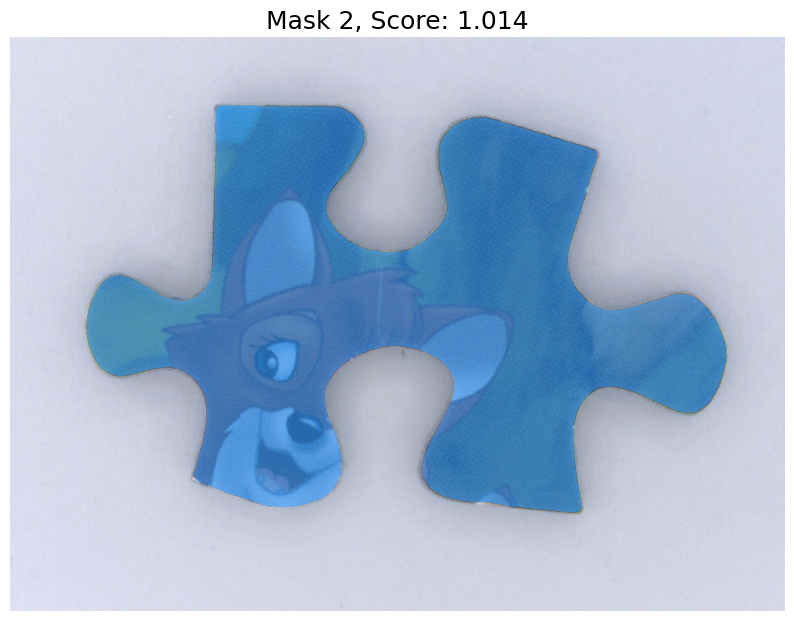
\includegraphics[width=0.4\textwidth]{sections/digitalize/images/scores_2.png}
    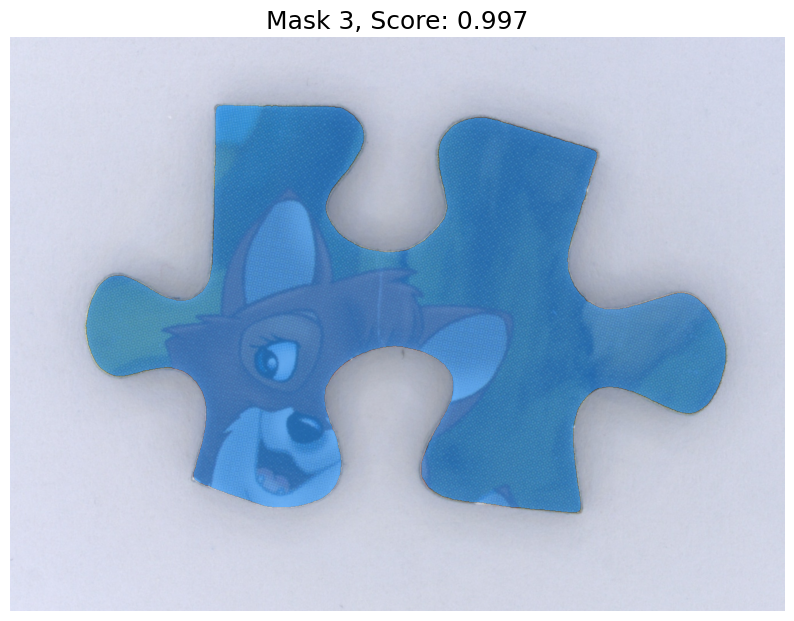
\includegraphics[width=0.4\textwidth]{sections/digitalize/images/scores_3.png}
    \caption{Ergebnisse der Multimask-Output-Bewertung in der Reihenfolge von Maske 1 (links), Maske 2 (rechts) und Maske 3 (unten)}
    \label{fig:sam_ergebnis}
\end{figure}

% Once the best mask is determined and the image is segmented, the mask is then saved and can be used for further processing with opencv. (continue to preprocessing)
Die Option "Multimask output" ist optional und standardmäßig aktiviert. Mit diesem Parameter kann SAM drei Masken ausgeben, zusammen mit der Einschätzung der Qualität dieser Masken durch das Modell. Diese Einstellung ist für mehrdeutige Aufforderungen gedacht, was hier nicht der Fall war. Es hat sich jedoch als vorteilhaft erwiesen, sie aktiviert zu lassen, da sie dem Modell mehr Spielraum (drei Masken) für genauere Vorhersagen lässt. Sobald der Inferenzprozess abgeschlossen ist, werden die segmentierten Masken zusammen mit ihren jeweiligen Punktzahlen angezeigt. Abbildung \ref{fig:sam_ergebnis} veranschaulicht die Ergebnisse, die durch einen einzigen Aufruf des \verb|predictor()| Funktion erzielt werden.
Die erhaltenen Segmentierungsmasken ermöglichen nun die Extraktion der optimalen Maske sowie den Beginn der Post-Processing-Phase.

In der Zusammenfassung lässt sich festhalten, dass SAM im Vergleich zur digitalen Bildverarbeitung ein qualitativ besseres Segmentierungsergebnis liefert. Es ist jedoch zu beachten, dass dieser Ansatz mit einem erheblichen Rechenaufwand verbunden ist. Dies wurde bei der anschließenden Portierung dieser Methode auf ROS noch deutlicher. Das Checkpoint-Modell war nicht für den mobilen Einsatz optimiert, was zu einer längeren Download-Zeit führte. Als nächste Herausforderung stellte sich das Laden des Modells in einen Docker-Container dar, um die notwendigen Inferenzen durchzuführen. Dies führte zum Auftreten von Speicherfehlern, die aufgrund der zeitlichen Beschränkungen des Projekts nicht behoben werden konnten. Ein alternativer Ansatz bestand darin, das Modell durch einen kleineren Modell-Checkpoint zu ersetzen. Die Qualität der Segmentierungsmaske, die durch diesen kleineren Checkpoint erzielt würde, konnte jedoch nicht evaluiert werden und wird daher lediglich als potenzielle Alternative oder als ein möglicher Ausblick auf die Zukunft zur Optimierung dieser Methode bezeichnet. 

\subsection[Postprocessing]{Postprocessing \myAuthor{Then}}

%common for both methodes:
Nachdem mit den oben genannten Methoden eine Segmentierungsmaske des gewünschten Objekts erstellt wurde, müssen die Ergebnisse nachbearbeitet werden, bevor sie den anderen Teams zur Verfügung gestellt werden können. Team Solver benötigt ein Bild des Puzzlestücks ohne Hintergrund (transparent), während Team Visualiser die Konturen der Puzzlestücke in einem reduzierten Format benötigt. In diesem Abschnitt wird beschrieben, wie ein Bild des Puzzlestücks mit transparentem Hintergrund (RGBA) und eine Maske der Konturen eines Puzzlestücks mit approximierten Kanten erstellt wird.

\subsubsection{Puzzleteil ohne Hintergrund (RGBA)}

%trimmed PNG figure here
%Figure of outputs here
\begin{figure}[h]
    \centering
    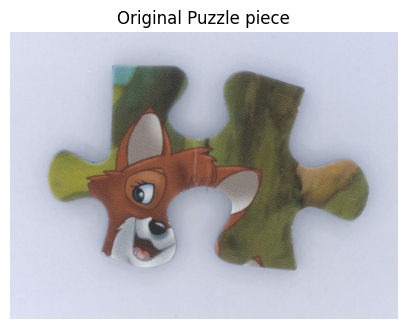
\includegraphics[width=0.4\textwidth]{sections/digitalize/images/original_trrimmed_1.png}
    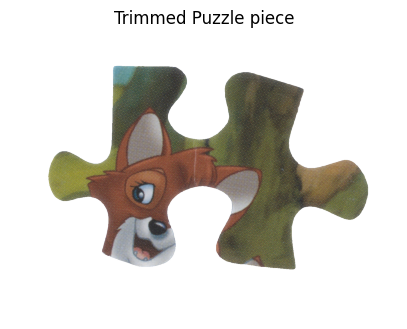
\includegraphics[width=0.4\textwidth]{sections/digitalize/images/original_trrimmed_2.png}
    \caption{Vor (links) und nach (rechts) dem Zuschneiden mit der Segmentierungsmaske}
    \label{fig:rgba_trim}
\end{figure}

%Vordergrund von Hintergrund trennen
Die Segmentierungsmaske liefert die Pixelpositionen in Form einer binären Maske des zu segmentierenden Bereichs. Um den Hintergrund zu entfernen, muss alles außer dem Puzzlestück identifiziert und entfernt werden. Zu diesem Zweck wird das Bild zunächst mit Hilfe der Bibliothek \verb|openCV| in vier Kanäle (RGBA) umgewandelt. Dann wird unter Verwendung der Pixelposition der erhaltenen Maske eine einfache Bedingung festgelegt, um den Alphakanal jeder Position außer der der Maske auf Null zu ändern. Das Ergebnis ist ein Bild, das nur aus dem Puzzleteil besteht. Das neu erhaltene Bild kann nun im PNG-Format gespeichert werden, das üblicherweise zum Speichern von Bildern mit vier Kanälen verwendet wird.

\subsubsection{Kanten Approximieren}

%warum sind viele kurze kanten blöd 
In ähnlicher Weise können die Konturen anhand der Position der Maske ermittelt werden. Die Konturen können mit der Funktion \verb|find_contours()| der Bibliothek \verb|scikit-image| \cite{scikit-image} gemessen werden, die die Maske als Eingabeparameter benötigt. Sie gibt die Kontur in Form von Pixelpositionen aus, die gegen x- und y-Koordinaten ausgetauscht werden müssen, damit sie in das Scalable Vector Graphics (SVG)-Format konvertiert werden können. Schließlich können die Pixelpositionen der Kontur in die SVG-Zeichnung eingefügt werden, so dass eine Datei entsteht, die nur die Konturen des Puzzlestücks enthält. Bei der Überprüfung der Ausgabe wurde jedoch ein wichtiges Problem festgestellt: Die Konturen waren zu detailliert. Wie bereits erwähnt, wurden die Pixelpositionen der Konturen direkt in die SVG-Datei eingefügt, was zu einer sehr detaillierten Kontur des Puzzlestücks führte. Die Einbeziehung so vieler Informationen würde den Rechenaufwand für die anschließende Visualisierung des Puzzleteils erheblich erhöhen, was nicht wünschenswert ist. 

% figure of approximated edges here 
\begin{figure}[h]
    \centering
    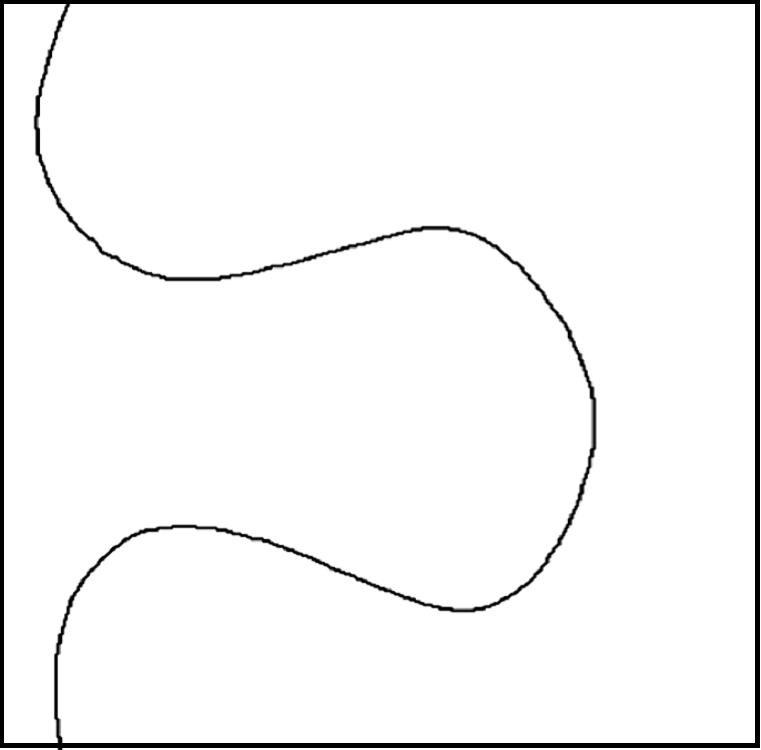
\includegraphics[width=0.4\textwidth]{sections/digitalize/images/rdp_before.png}
    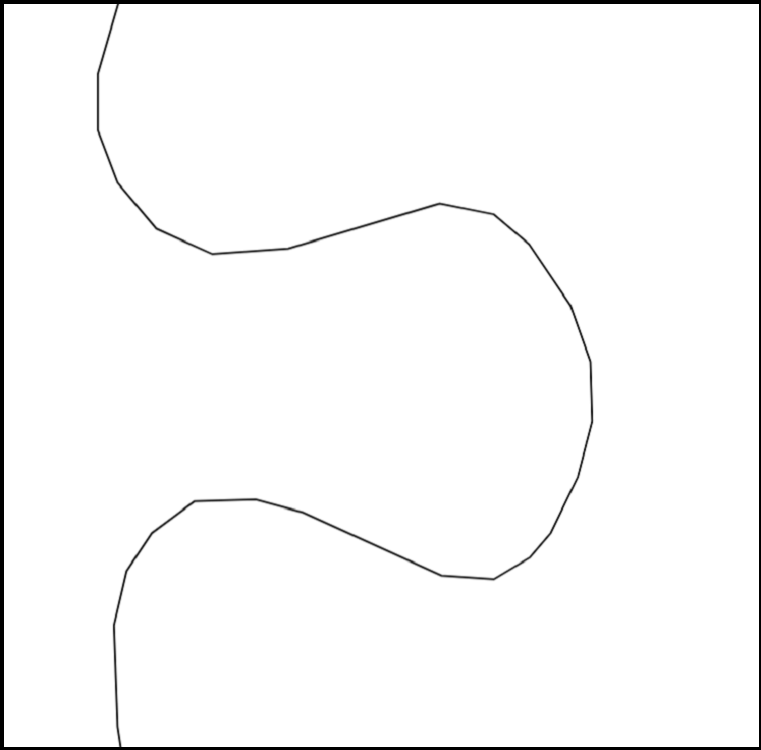
\includegraphics[width=0.4\textwidth]{sections/digitalize/images/rdp_after.png}
    \caption{Vergleich von vor (links) und nach (rechts) der Approximierung}
    \label{fig:kanten_approx}
\end{figure}
%dafür kanten approximieren, wenige kurze kanten
%rdp algorithm macht genau das
Um dieses Problem zu lösen, müssen die Kanten einer Form der Merkmalsreduktion unterzogen werden. Der Ramer-Douglas-Peucker-Algorithmus (RDP) \cite{douglas1973algorithms} wurde eingesetzt, um die Anzahl der Punkte in einer durch eine Reihe von Punkten approximierten Kurve zu reduzieren. Abbildung \ref{fig:kanten_approx} zeigt die Ergebnisse bei der Verringerung der Anzahl der Punkte, die erforderlich sind, um den Großteil der Krümmung an den Kanten der Konturen zu erhalten. Mit den neu erhaltenen approximierten Kanten kann diese schließlich in der endgültigen SVG-Datei gespeichert werden.

\subsection[ROS-Node]{ROS-Node \myAuthor{Kipp}}
Das Projekt schreibt vor, dass die Teilkomponenten Digitalizer, Solver, Controller und Visulizer über das Roboter Operation System, kurz ROS, kommunizieren.
Das hat unter anderem den Vorteil, dass der ROS-Node, welcher die Segmentierung mit KI durchführt, auf einer sehr leistungsstarken Hardware laufen kann, während andere Nodes auf sparsamer Hardware oder verteilt laufen können.
Durch ROS ist also das Übertragungsprotokoll definiert, die Interfaces zwischen den Nodes müssen unter enger Abstimmung selbst definiert und eingehalten werden.
Der Digitalize-Node hat eine Schnittstelle zu dem Solver- und dem Visualisierungs-Node.
Die Solver fragen den Digitalizer nach segmentierten Puzzleteile, um das Puzzle zu lösen und die Visualizer wollen die segmentierten Puzzleteile anzeigen, sobald es vom Roboter bewegt wird.

\subsubsection{Kommunikation}
Es muss sichergestellt werden, dass der Solver alle Puzzleteile empfängt oder zumindest überprüfen kann, ob Bilder vollständig sind.
ROS2 beinhaltet \textit{Action Server}, welche von einem Client mit einem Request bzw. Goal aufgerufen werden können.
Der Action Server entscheidet dann, ob das Goal akzeptiert wird und sendet ein Acknowledgement an den Client.
Daraufhin kann der Action Server das Goal ausführen und während dessen Feedback an den Client schicken.
Sobald das Goal erreicht wurde, wird eine Response verschickt.
Dieses Actionprotokoll kann gut auf den Segmentierungsvorgang übertragen werden.
So sendet der Solver eine \verb|digitalize/segment| Action an den Digitializer-Node mit den Request, Puzzleteile zu segmentieren.
Der Digitalizer kann daraufhin mit der Segmentierung beginnen und sobald Puzzelteile fertig sind, diese als Feedback an den Solver verschicken.
Ist die Übertragung beendet, wird eine Response versendet mit der der Solver überprüfen kann, ob alle Bilder korrekt empfangen wurden und daraufhin das Puzzle lösen.
In Sequenzdiagramm von Abbildung \ref{fig:ros_digi_seq} ist die Action oben zu sehen.

Die Visualizer bekommen von Control Bewegungskommandos und dazugehörige Puzzelteil IDs.
Sie brauchen also ebenfalls alle Puzzelteile, können sich jedoch nicht auf die Feedback-Topic der Segmentierungs-Action subscriben.
Für das Just-In-Time Mapping von neuen IDs zu Puzzleteilen wäre ein REST-API Endpunkt ähnlicher Get Request über einen ROS-Service denkbar gewesen, der Einfachheit halber wurde aber eine Topic \verb|digitalize/imgs| eingerichtet, auf welcher nach erfolgreicher Segmentierung alle Puzzleteile publiziert werden.
Das hat den Vorteil, dass der Visualize-Node nur auf die Topic subscriben muss und sofort alle Bilder im Speicher hat.
Ein entsprechendes Publish-Verhalten ist im Sequenzdiagramm \ref{fig:ros_digi_seq} zu sehen.

\begin{figure}[h]
    \centering
    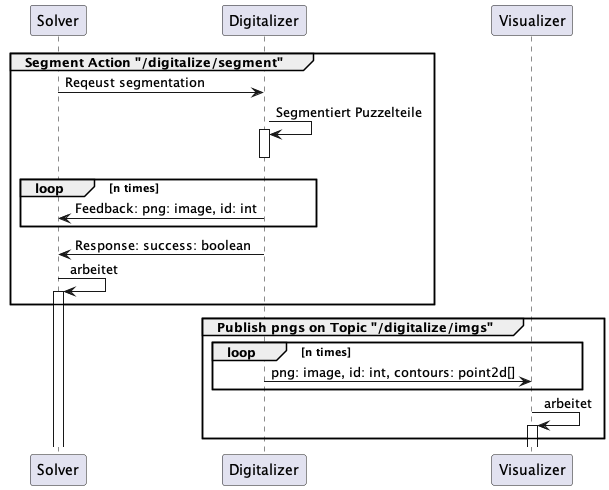
\includegraphics[width=0.9\textwidth]{sections/digitalize/images/ros_pkg_digi_seq.png}
    \caption{Sequenzdiagramm Kommunikation}
    \label{fig:ros_digi_seq}
\end{figure}

\subsubsection{Interfaces}
Für den Solver ist es wichtig, das Puzzleteil als PNG zu bekommen, sowie eine ID als Integer.
ROS stellt mit Message \verb|sensor_msgs/Image| bereits eine Möglichkeit bereit, wie Bilder verschickt werden könne.
Das Segmentierungs-Goal muss nicht weiter definiert werden, da klar ist, was zu tun ist.
Ob alle Puzzleteile empfangen worden sind, kann überprüft werden, indem die Response die Anzahl der versendeten Bilder beinhaltet.
Demgemäß ergibt sich folgende Schnittstelle von Digitalize zu Solver für die Segment-Action:
\begin{verbatim}
                      # Request
---
int32 png_total_count # Response
---
sensor_msgs/Image png # Feedback
int32 id # Feedback
\end{verbatim}

Die Kommunikation zwischen Visualize und Digitalize basiert auf einfachen Topics, die jederzeit versendet werden können, eine einfach ROS Message ist also ausreichend.
Zusätzlich zu dem Puzzle PNG und der ID, benötigen der Visualize-Node noch die Konturen des Puzzleteils, um dieses Triangulieren zu können.
Die Konturen werden als Liste von $(x, y)$ Koordinaten versendet.
Daraus ergibt sich folgende Schnittstelle von Digitalize zu Visualize für den Image-Publisher:
\begin{verbatim}
int32 id
sensor_msgs/Image png
Point2d[] points
\end{verbatim}

Wobei \verb|Point2d| wie folgt definiert ist:
\begin{verbatim}
int32 x
int32 y
\end{verbatim}

\subsubsection{Architektur}
Der Digitalize ROS2 Node ist mit hilfe der \verb|rclpy|, ein ROS Package, ebenfalls in Python geschrieben.
Die Architektur kann dem Diagramm \ref{fig:ros_digi_arch} entnommen werden.
Der \verb|manager| wird ist der Entry-Point in den node, wird also mit \verb|ros2 run pgk_digitalize manager| gestartet.
Dieser wiederum registriert  den Segment Action Server und den Image Publisher.
Segmentiert wird entweder mit der mit reiner Bildverarbeitung oder mit KI.

\begin{figure}[h]
    \centering
    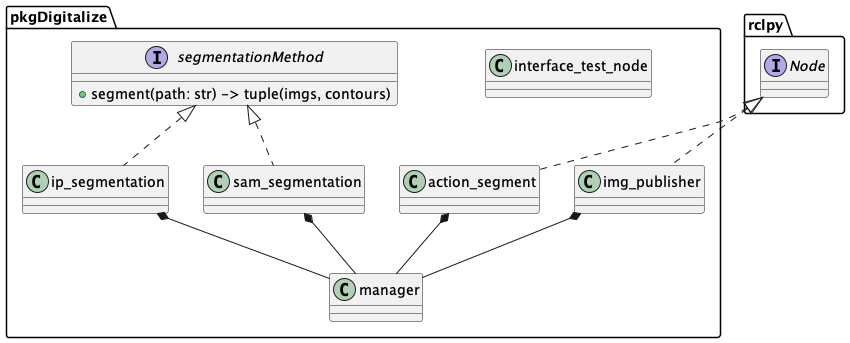
\includegraphics[width=0.9\textwidth]{sections/digitalize/images/ros_pgk_digi_class.png}
    \caption{Digitalize ROS Node Architektur}
    \label{fig:ros_digi_arch}
\end{figure}
